\section{برنامه ریزی}
در این بخش به برسی موجودیت های کلی سیستم و PRD های نسخه اولیه سیستم می‌پردازیم.

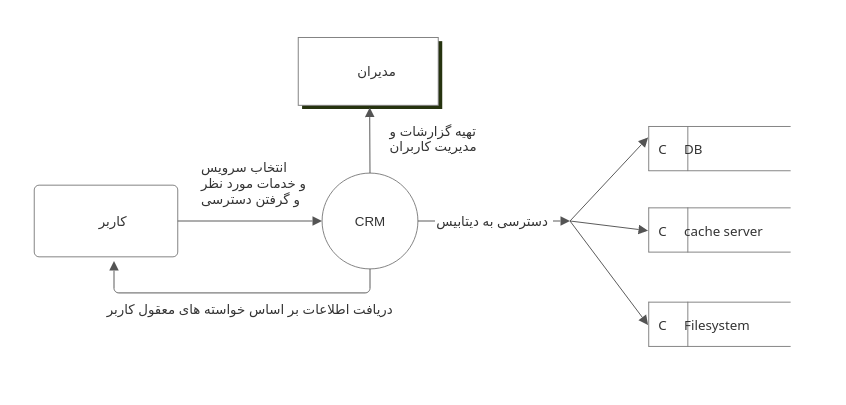
\includegraphics[scale=0.8]{assets/0_level_system.png}

سیستم سطح صفر، و انتزاعی ترین مدل سیست به صورت نمودار DFD فوق است.
کاربر وارد سیستم شده و بر اساس سطوح دسترسی خود حق انتخاب سرویس های مورد نظر خود را خواهد داشت. بعد از آن
داده های خود را بواسطه سیستم در دیتابیس های مختلفی می‌تواند ذخیره کند.
برای مثال رکورد های دیتابیس در Postgres ذخیره شده، برخی لاگ ها یا رویداد ها بواسطه Redis منتقل شده و مستندات بصورت فایل داخل سرور قرار می‌گیرند.

در کنار این روند کلی، مدیران سطوح بالا تر و خود کاربران می‌توانند داده های بسیاری را در سیستم مشاهده کنند.

سیستم به زیر سیستم های مختلفی تقسیم می‌شود که به آنها خواهیم پرداخت.

\subsection{زیر سیستم احراز هویت}
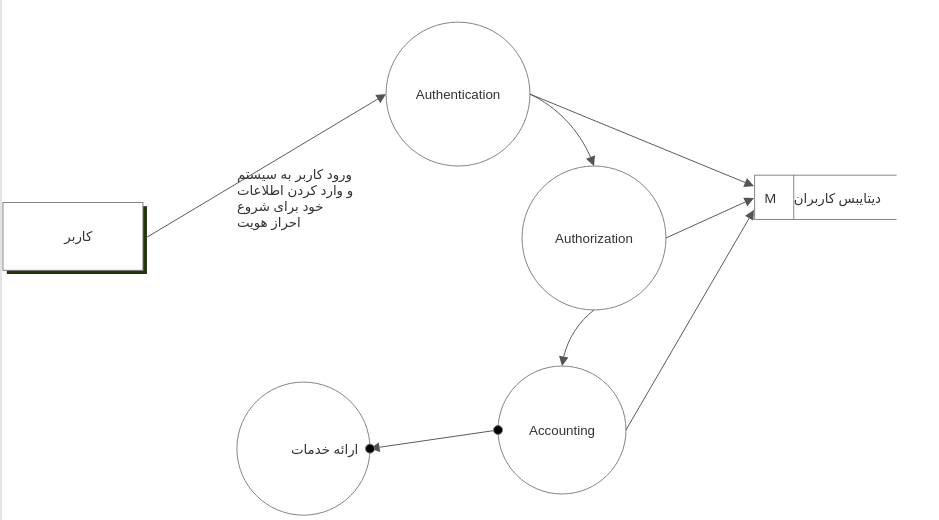
\includegraphics[scale=0.8]{assets/auth_dfd.png}
نمودار DFD مرتبط با احراز هویت کاربران به این شکل می‌باشد.
مراحل احراز هویت با جزئیات بیشتر توضیح داده خواهد شد:

\begin{itemize}
	\item کاربر ابتدا مشخصات خود را در سیستم وارد می‌کند.
	\item سیستم طی مرحله ای به نام Authentication تشخیص می‌دهد که آیا کاربر اجازه ورود به سیستم دارد یا خیر.
	\item بعد از آن سیستم در مرحله Authorization مشخص می‌کند که کاربر به چه بخش هایی از سیستم می‌تواند دسترسی داشته باشد.
	\item بخش دیگری از سیستم با نام Accounting در حین استفاده کاربر از سیستم، گزارشاتی را طهیه خواهد کرد و برای مدیریان سطح بالا تر ارسال می‌کند.
	\item در نهایت نیز کاربر می‌تواند به سرویس دلخواه و قابل دسترس خود دست پیدا کند.
\end{itemize}

در نمودار ERD زیر به موجودیت ها و صفات موجود در کاربر ها و role هایشان می‌پردازیم.

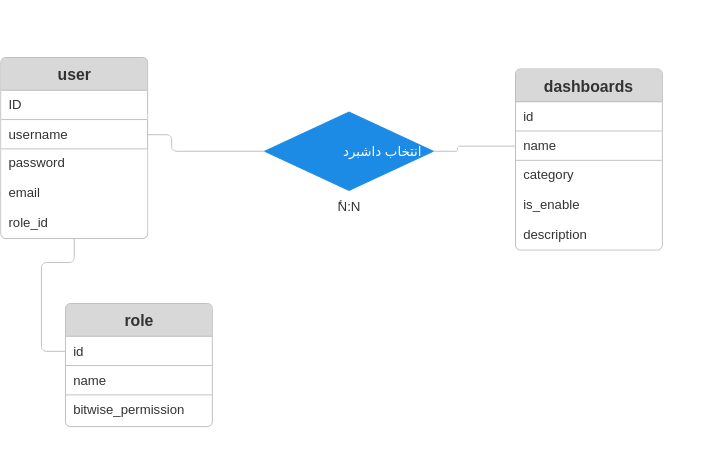
\includegraphics[scale=0.8]{assets/auth_erd.png}

همانطور که مشاهده می‌کنید، هر کاربر یک role دارد. این مقادیر را سیستم در حین احراز هویت از دیتابیس دریافت کرده و بر اساس آن انتخاب می‌کند
کدام کاربر حق ورود به چه زیر سیستم هایی را دارد.

\subsection{زیر سیستم حساب داری}

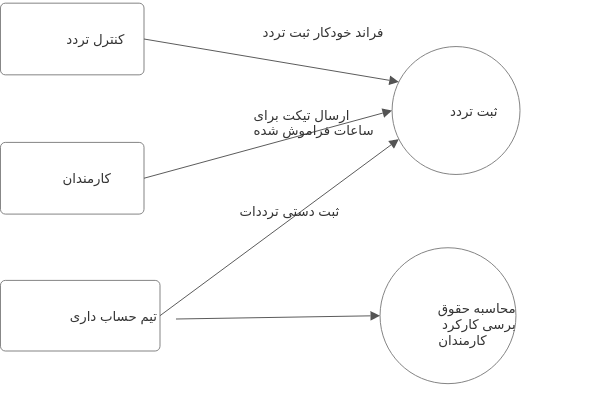
\includegraphics[scale=0.8]{assets/finance_dfd.png}

زیر سیستم حساب داری دو وظیفه مهم را بر عهده دارد. تیم های مختلف می‌توانند از طریق این زیر سیستم تردد و گزارشات مرتبط به آن را دنبال کنند.
روزانه کارمندان بواسطه دستگاه تردد، ورود و خروج های خود را ثبت می‌کنند.
این سیستم به دستگاه ثبت تردد متصل بوده و این تردد ها را به صورت خودکار داخل دیتابیس ثبت خواهد کرد.
در صورتی که فرد فراموش کرده بود، می‌تواند به مدیران حساب داری و منابع انسانی اطلاع دهد. این مدیران به صورت مستقیم
توانایی و اجازه ویرایش و اضافه کردن رکورد به دیتابیس ورود و خروج دارند.
راه دیگر آنها نیز تیکت زدن به واحد مدیریت خواهد بود.

زیر سیستم حساب داری بیشتر خدمات خود را به واحد منابع انسانی خواهد داد. به طوری که در داشبرد منابع انسانی، می‌تواند برای کارمندان
حقوق و الگوریتم محاسبه آن تعریف شود. در کنار آن گرفتن مرخصی و بثبت پرداختی ها از همین بخش انجام خواهد شد.

\subsection{زیر سیستم مدیریت پروژه}
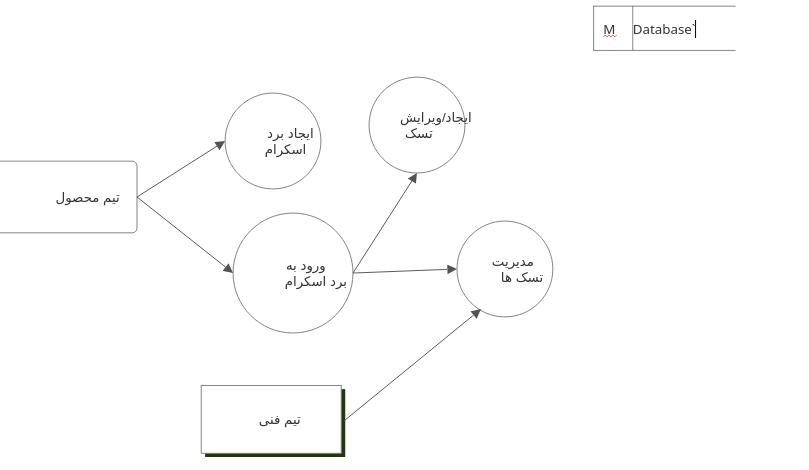
\includegraphics[scale=0.8]{assets/product_dfd.png}

تیم محصول می‌تواند برد های مورد نیاز خود را ایجاد کند و تسک های لازم را برای بستتن اسپرینت ها و استفاده از اسکرام تعریف کند.
تیم فنی نیز می‌تواند تسک های خود را دنبال کند، و وضعیت آنها را بر اساس آنچه که باید تغییر بدهد. تیم فنی باید تخمین های زمانی و زمان سپری کرده روی هر تسک را 
در این زیر سیستم مشخص کند.
تیم فنی و محصول هر  زمان بخواهند می‌توانند گزارشات مرتبط با عملکرد کاری خود را مشاهده کنند.
اما تیم محصول گزارشات بیشتری خواهند داشت.
برای مثال اگر توسعه دهنده ای بیش از حد تسک هایی داشته باشد که زمان سپری شده آنها بیش از زمان تخمین زده باشد، به مدیر محصول اخطار داده می‌شود.
تمام داده ها در دیتابیس ذخیره شده و مجددا می‌تواند مورد استفاده قرار گیرد.

\subsection{زیر سیستم مستند سازی}
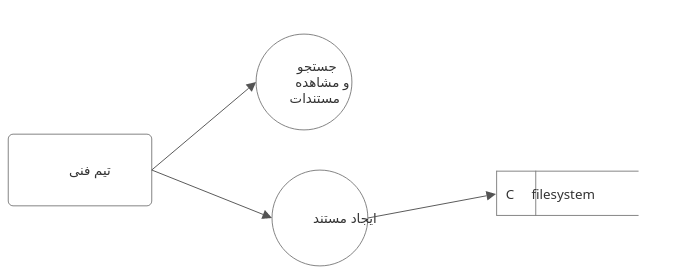
\includegraphics[scale=0.8]{assets/doc_dfd.png}

تیم فنی می‌تواند بر اساس دسترسی خود مستنداتی بسازد و باقی تیم نیز بر اساس سطوح دسترسی به مستندان فنی مختلف دسترسی داشته باشند.
نکته حائز اهمیت در این سیستم، امنیت و سطوح دسترسی آن خواهد بود. مدیران بالا تر می‌توانند دسته بندی و پروژه های مختلف تعریف کنند و به نیرو های دیگر
بر اساس نیاز دسترسی های مختلف بدهد.
کاربر می‌تواند فقط دسترسی دیدن مستندات خاصی را داشته باشد یا بتواند آنها را ویرایش یا حذف کند.

ادمین و سازنده هر مستند می‌تواند لیست افرادی که به آن دسترسی دارد را کنترل کند. این لیست درواقع به جدول role مرتبط است که قبل تر به آن اشاره شده.

\subsection{زیر سیستم مدیریت تنظیمات}
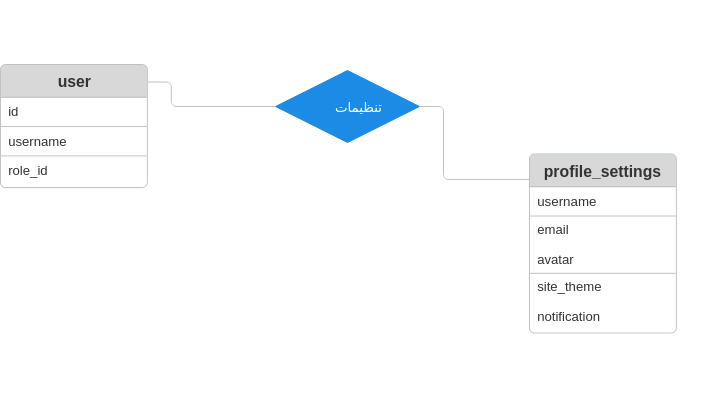
\includegraphics[scale=0.8]{assets/settings_erd.png}

کاربرات از بخش تنظیمات می‌توانند اطلاعات کلی حساب کاربری خود را ویرایش کنند. از این بخش، نام، ایمیل و عکس پروفایل خود را می‌توانند تغییر دهند.
همچنان تم سایت و اینکه نوتیفیکیشن ارسال بشود یا خیر قابل تنظیم است.

\subsection{زیر سیستم مانیتورینگ}
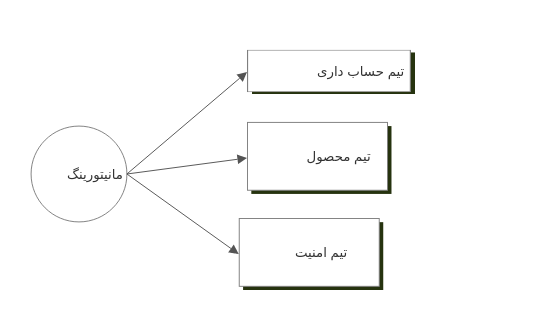
\includegraphics[scale=0.8]{assets/monitoring_dfd.png}
رخداد ها و اتفاق هایی در سیستم وجود دارد که سیستم می‌تواند آنها را به کاربران اعلان کند و از مشکلات و اتفاقاتی خبر دار کند.
سیستم مانیتورینگ به هر دسته و سطوح دسترسی خاص، بر اساس وظایف آنها یک سری لاگ ها و اعلان ها را ارسال می‌کنید.

\subsubsection{اعلان های سیستم مانیتورینگ برای تیم حساب داری}
\begin{itemize}
	\item غایب بودن یک نیرو خاص
	\item وجود کسری کار غیر معقول برای یک شخص
	\item دیر شدن در پرداختی های کارمند ها 
\end{itemize}

\subsubsection{اعلان های سیستم مانیتورینگ برای تیم محصول}
\begin{itemize}
	\item نرسیدن تسک ها با اسپرینت
	\item ثبت غیر معقول زمان سپری شده روی یک تسک برای کاربری خاص
	\item گزارشات ناقص یک کاربر
	\item تغییر مثبت و منفی یک نیرو در بازه زمانی خاص
\end{itemize}

\subsubsection{اعلان های سیستم مانیتورینگ برای تیم امنیت}
\begin{itemize}
	\item تلاش کاربر نا شناخته برای ورود به سیستم
	\item محدود بودن منابع سرور و خطر
	\item حمله ای از سمت یک کاربر ناشناخته درحال انجام است
\end{itemize}
